\documentclass{standalone}
\usepackage[utf8]{inputenc}
\usepackage[T1]{fontenc}
\usepackage{tikz}
\usepackage{amsmath}
\usepackage{xcolor}

\begin{document}
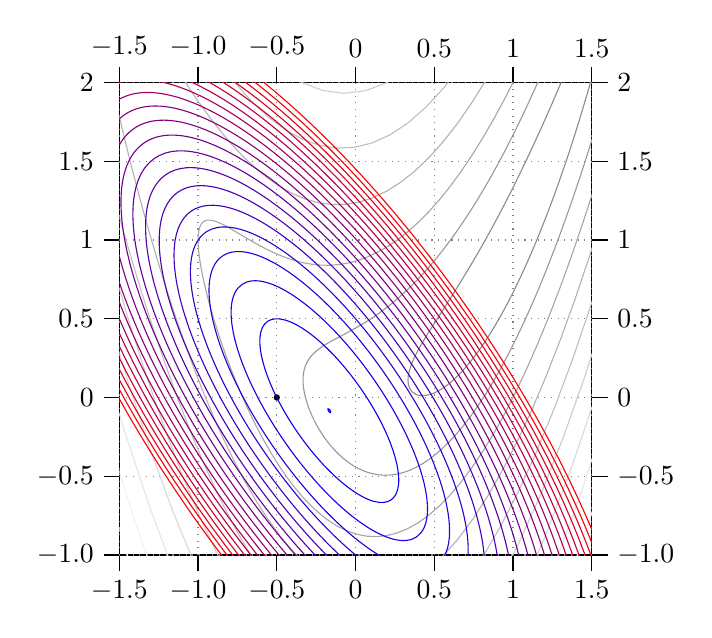
\begin{tikzpicture}[scale=2]
\def\xm{-1.5}
\def\xs{0.5}
\def\xM{1.5}
\def\ym{-1.0}
\def\ys{0.5}
\def\yM{2.0}
\pgfmathsetmacro\xmps{\xm+\xs}
\pgfmathsetmacro\ymps{\ym+\ys}
\def\a{7}
\def\b{8}
\def\c{4}
\def\d{3}
\def\e{2}
\def\f{2.25}
\def\minlevel{1.917}
\def\levelset{2.5}
\pgfmathsetmacro\Delta{(\a-\c)*(\a-\c)+\b*\b}
\pgfmathsetmacro\M{(\a+\c+sqrt(\Delta))/2}
\pgfmathsetmacro\m{(\a+\c-sqrt(\Delta))/2}
\pgfmathsetmacro\ang{atan2(2*(\M-\a)/\b, 1.0)}
\pgfmathsetmacro\di{\d*cos(\ang) + \e*sin(\ang)}
\pgfmathsetmacro\ei{-\d*sin(\ang) + \e*cos(\ang)}
\pgfmathsetmacro\Cx{-\di/(2*\M)}
\pgfmathsetmacro\Cy{-\ei/(2*\m)}
  \draw (\xm,\ym) rectangle (\xM,\yM);
  \foreach \x in {\xm,\xmps,...,\xM} {
    \draw (\x,\ym) -- (\x,\ym-0.1) node[below] {$\x$};
    \draw (\x,\yM) -- (\x,\yM+0.1) node[above] {$\x$};
    \draw[gray,dotted] (\x,\ym) -- (\x,\yM);
  }
  \foreach \y in {\ym,\ymps,...,\yM} {
    \draw (\xm,\y) -- (\xm-0.1,\y) node[left] {$\y$};
    \draw (\xM,\y) -- (\xM+0.1,\y) node[right] {$\y$};
    \draw[gray,dotted] (\xm,\y) -- (\xM,\y);
  }
  \clip (\xm,\ym) rectangle (\xM,\yM);

  \fill (-0.5,0) circle (0.02);
  \foreach \L in {0, 10, ..., 100} {
    \pgfmathsetmacro\r{\L/15}
    \draw[domain=0:360, samples=180, color=white!\L!gray] plot
       ({1-\r*cos(\x)}, {1 -2*\r*cos(\x) + \r*\r*cos(\x)*cos(\x) + \r*sin(\x)/2});
  }
  \foreach \L in {0, 5, ..., 100} {
    \pgfmathsetmacro\r{\minlevel + (\L/5)*(\levelset-\minlevel)}
    \pgfmathsetmacro\F{\r-\f+\di*\di/(4*\M)+\ei*\ei/(4*\m)}
    \pgfmathsetmacro\rx{sqrt(\F/\M)}
    \pgfmathsetmacro\ry{sqrt(\F/\m)}
    \draw[rotate=\ang, shift={(\Cx,\Cy)}, color=red!\L!blue]
      (0,0) ellipse ({\rx} and {\ry});
   }
\end{tikzpicture}
\end{document}
